% ================================================================
% EMPIRICAL APPLICATION — Dominick's Analgesics
% Auto-generated by run_dominicks_experiments.py
% n\_runs = 2  (mean $\pm$ std across independent re-estimations)
% Packages: booktabs, threeparttable, graphicx, siunitx
% ================================================================

\begin{table}[htbp]
  \centering
  \caption{Descriptive Statistics: Dominick's Analgesics Scanner Panel}
  \label{tab:dom_desc}
  \begin{threeparttable}
    \begin{tabular}{lS[table-format=2.3]S[table-format=1.3]S[table-format=1.4]S[table-format=1.4]}
      \toprule
      \textbf{Good} & {\textbf{Mean Price}} & {\textbf{Std Price}} & {\textbf{Mean Share}} & {\textbf{Std Share}} \\
      & {(\$/100 tablets)} & & & \\
      \midrule
      Aspirin & 7.311 & 1.557 & 0.2107 & 0.0519 \\
      Acetaminophen & 10.554 & 1.427 & 0.5026 & 0.0785 \\
      Ibuprofen & 10.506 & 1.428 & 0.2867 & 0.0819 \\
      \midrule
      \multicolumn{5}{l}{\textit{Train: 28,644 obs\quad Test: 4,287 obs\quad Stores: 93\quad Weeks: 1--399}} \\
      \bottomrule
    \end{tabular}
    \begin{tablenotes}\small
      \item Unit prices standardised to per-100-tablet equivalent.
    \end{tablenotes}
  \end{threeparttable}
\end{table}

\begin{table}[htbp]
  \centering
  \caption{Out-of-Sample Predictive Accuracy --- Dominick's Analgesics (2 independent re-estimations; mean $\pm$ std)}
  \label{tab:dom_acc}
  \begin{threeparttable}
    \begin{tabular}{lcc}
      \toprule
      \textbf{Model} & \textbf{RMSE} & \textbf{MAE} \\
      \midrule
      LA-AIDS & $0.07069 \pm 0.00000$ & $0.05593 \pm 0.00000$ \\
      BLP (IV) & $0.07766 \pm 0.00000$ & $0.05991 \pm 0.00000$ \\
      QUAIDS & $0.06956 \pm 0.00000$ & $0.05519 \pm 0.00000$ \\
      \textbf{Series Est.} & \textbf{$0.06514 \pm 0.00000$} & $0.05077 \pm 0.00000$ \\
      Neural Demand (window) & $0.08635 \pm 0.00008$ & $0.06855 \pm 0.00210$ \\
      LDS (Shared) & $0.09237 \pm 0.00000$ & $0.07426 \pm 0.00000$ \\
      LDS (GoodSpec) & $0.09242 \pm 0.00000$ & $0.07436 \pm 0.00000$ \\
      LDS (Orth) & $0.09291 \pm 0.00000$ & $0.07485 \pm 0.00000$ \\
      Neural Demand (static) & $0.08778 \pm 0.00197$ & $0.06872 \pm 0.00155$ \\
      Neural Demand (habit) & $0.07466 \pm 0.00023$ & $0.05803 \pm 0.00069$ \\
      Neural Demand (FE) & $0.08703 \pm 0.00133$ & $0.06787 \pm 0.00099$ \\
      Neural Demand (habit, FE) & $0.08047 \pm 0.00296$ & $0.06258 \pm 0.00249$ \\
      Neural Demand (CF) & $0.08557 \pm 0.00035$ & $0.06691 \pm 0.00012$ \\
      Neural Demand (habit, CF) & $0.06969 \pm 0.00536$ & $0.05382 \pm 0.00480$ \\
      Neural Demand (habit, FE, CF) & $0.07869 \pm 0.00067$ & $0.06151 \pm 0.00079$ \\
      Neural Demand (placebo) & $0.08440 \pm 0.00366$ & $0.06611 \pm 0.00243$ \\
      \bottomrule
    \end{tabular}
    \begin{tablenotes}\small
      \item RMSE and MAE on held-out test observations, mean $\pm$ std over 2 run(s).
    \end{tablenotes}
  \end{threeparttable}
\end{table}

\begin{table}[htbp]
  \centering
  \caption{Own-Price Quantity Elasticities --- Dominick's Analgesics (2 run(s); mean $\pm$ std)}
  \label{tab:dom_elast}
  \begin{threeparttable}
    \begin{tabular}{lccc}
      \toprule
      \textbf{Model} & {$\hat{\varepsilon}_{00}$ (Aspirin)} & {$\hat{\varepsilon}_{11}$ (Acetaminophen)} & {$\hat{\varepsilon}_{22}$ (Ibuprofen)} \\
      \midrule
      LA-AIDS & $-0.849 \pm 0.000$ & $-1.420 \pm 0.000$ & $-1.140 \pm 0.000$ \\
      BLP (IV) & $-0.998 \pm 0.000$ & $-1.769 \pm 0.000$ & $-0.587 \pm 0.000$ \\
      QUAIDS & $-0.882 \pm 0.000$ & $-1.423 \pm 0.000$ & $-1.129 \pm 0.000$ \\
      Series Est. & $-0.708 \pm 0.000$ & $-1.629 \pm 0.000$ & $-1.224 \pm 0.000$ \\
      Neural Demand (window) & $-1.006 \pm 0.028$ & $-0.995 \pm 0.003$ & $-1.020 \pm 0.010$ \\
      LDS (Shared) & $-0.202 \pm 0.000$ & $-0.241 \pm 0.000$ & $-0.219 \pm 0.000$ \\
      LDS (GoodSpec) & $-0.210 \pm 0.000$ & $-0.240 \pm 0.000$ & $-0.220 \pm 0.000$ \\
      LDS (Orth) & $-0.536 \pm 0.000$ & $-0.640 \pm 0.000$ & $-0.499 \pm 0.000$ \\
      Neural Demand (static) & $-0.948 \pm 0.083$ & $-0.929 \pm 0.009$ & $-1.028 \pm 0.035$ \\
      Neural Demand (habit) & $-1.010 \pm 0.137$ & $-0.988 \pm 0.024$ & $-1.045 \pm 0.014$ \\
      Neural Demand (FE) & $-1.059 \pm 0.054$ & $-0.951 \pm 0.019$ & $-1.050 \pm 0.017$ \\
      Neural Demand (habit, FE) & $-1.055 \pm 0.044$ & $-0.973 \pm 0.006$ & $-1.012 \pm 0.004$ \\
      Neural Demand (CF) & $-1.007 \pm 0.010$ & $-0.970 \pm 0.002$ & $-1.074 \pm 0.006$ \\
      Neural Demand (habit, CF) & $-1.018 \pm 0.061$ & $-1.044 \pm 0.037$ & $-0.995 \pm 0.001$ \\
      Neural Demand (habit, FE, CF) & $-1.031 \pm 0.051$ & $-0.946 \pm 0.009$ & $-0.994 \pm 0.023$ \\
      Neural Demand (placebo) & $-0.991 \pm 0.019$ & $-0.948 \pm 0.004$ & $-1.045 \pm 0.045$ \\
      \bottomrule
    \end{tabular}
    \begin{tablenotes}\small
      \item Numerical own-price quantity elasticities at mean test prices.
    \end{tablenotes}
  \end{threeparttable}
\end{table}

\begin{table}[htbp]
  \centering
  \caption{Consumer Surplus Loss from 10\% Ibuprofen Price Increase --- Dominick\'s Analgesics (2 run(s); mean $\pm$ std)}
  \label{tab:dom_welfare}
  \begin{threeparttable}
    \begin{tabular}{lcr}
      \toprule
      \textbf{Model} & \textbf{CV Loss (\$)} & \textbf{vs Neural Demand (static)} \\
      \midrule
      LA-AIDS & $-0.2322 \pm 0.0000$ & +0.3\% \\
      BLP (IV) & $-0.2212 \pm 0.0000$ & +5.0\% \\
      QUAIDS & $-0.2339 \pm 0.0000$ & -0.5\% \\
      Series Est. & $-0.2333 \pm 0.0000$ & -0.2\% \\
      Neural Demand (window) & $-0.2313 \pm 0.0053$ & +0.7\% \\
      LDS (Shared) & $-0.2857 \pm 0.0000$ & -22.7\% \\
      LDS (GoodSpec) & $-0.2860 \pm 0.0000$ & -22.8\% \\
      LDS (Orth) & $-0.2561 \pm 0.0000$ & -10.0\% \\
      Neural Demand (static) & $-0.2328 \pm 0.0031$ &  \\
      Neural Demand (habit) & $-0.2277 \pm 0.0048$ & +2.2\% \\
      Neural Demand (FE) & $-0.2276 \pm 0.0016$ & +2.2\% \\
      Neural Demand (habit, FE) & $-0.2292 \pm 0.0006$ & +1.6\% \\
      Neural Demand (CF) & $-0.2309 \pm 0.0006$ & +0.8\% \\
      Neural Demand (habit, CF) & $-0.2270 \pm 0.0064$ & +2.5\% \\
      Neural Demand (habit, FE, CF) & $-0.2318 \pm 0.0023$ & +0.5\% \\
      Neural Demand (placebo) & $-0.2314 \pm 0.0032$ & +0.6\% \\
      \bottomrule
    \end{tabular}
    \begin{tablenotes}\small
      \item Compensating variation via 100-step Riemann sum, $p_{\mathrm{Ibu}}\to(1+0.1)\,p_{\mathrm{Ibu}}$.
    \end{tablenotes}
  \end{threeparttable}
\end{table}

\begin{table}[htbp]
  \centering
  \caption{Consumer Surplus Loss from 10\% Aspirin Price Increase --- Dominick\'s Analgesics (2 run(s); mean $\pm$ std)}
  \label{tab:dom_welfare_aspirin}
  \begin{threeparttable}
    \begin{tabular}{lcr}
      \toprule
      \textbf{Model} & \textbf{CV Loss (\$)} & \textbf{vs Neural Demand (static)} \\
      \midrule
      LA-AIDS & $-23.2182 \pm 0.0000$ & +0.3\% \\
      BLP (IV) & $-22.1176 \pm 0.0000$ & +5.0\% \\
      QUAIDS & $-23.3916 \pm 0.0000$ & -0.5\% \\
      Series Est. & $-23.3300 \pm 0.0000$ & -0.2\% \\
      Neural Demand (window) & $-23.1251 \pm 0.5316$ & +0.7\% \\
      LDS (Shared) & $-28.5654 \pm 0.0000$ & -22.7\% \\
      LDS (GoodSpec) & $-28.5995 \pm 0.0000$ & -22.8\% \\
      LDS (Orth) & $-25.6126 \pm 0.0000$ & -10.0\% \\
      Neural Demand (static) & $-23.2837 \pm 0.3143$ &  \\
      Neural Demand (habit) & $-22.7662 \pm 0.4805$ & +2.2\% \\
      Neural Demand (FE) & $-22.7648 \pm 0.1614$ & +2.2\% \\
      Neural Demand (habit, FE) & $-22.9153 \pm 0.0627$ & +1.6\% \\
      Neural Demand (CF) & $-23.0939 \pm 0.0551$ & +0.8\% \\
      Neural Demand (habit, CF) & $-22.6953 \pm 0.6354$ & +2.5\% \\
      Neural Demand (habit, FE, CF) & $-23.1786 \pm 0.2282$ & +0.5\% \\
      Neural Demand (placebo) & $-23.1435 \pm 0.3189$ & +0.6\% \\
      \bottomrule
    \end{tabular}
    \begin{tablenotes}\small
      \item Compensating variation via 100-step Riemann sum, $p_{Aspirin}\to(1+0.1)\,p_{Aspirin}$.
    \end{tablenotes}
  \end{threeparttable}
\end{table}

\begin{table}[htbp]
  \centering
  \caption{Consumer Surplus Loss from 10\% Acetaminophen Price Increase --- Dominick\'s Analgesics (2 run(s); mean $\pm$ std)}
  \label{tab:dom_welfare_acetaminophen}
  \begin{threeparttable}
    \begin{tabular}{lcr}
      \toprule
      \textbf{Model} & \textbf{CV Loss (\$)} & \textbf{vs Neural Demand (static)} \\
      \midrule
      LA-AIDS & $-53.2076 \pm 0.0000$ & +10.0\% \\
      BLP (IV) & $-47.9725 \pm 0.0000$ & +18.8\% \\
      QUAIDS & $-52.9144 \pm 0.0000$ & +10.5\% \\
      Series Est. & $-51.2835 \pm 0.0000$ & +13.2\% \\
      Neural Demand (window) & $-58.4197 \pm 0.7220$ & +1.2\% \\
      LDS (Shared) & $-46.1529 \pm 0.0000$ & +21.9\% \\
      LDS (GoodSpec) & $-46.1298 \pm 0.0000$ & +21.9\% \\
      LDS (Orth) & $-57.0314 \pm 0.0000$ & +3.5\% \\
      Neural Demand (static) & $-59.1013 \pm 0.2168$ &  \\
      Neural Demand (habit) & $-57.0165 \pm 0.4820$ & +3.5\% \\
      Neural Demand (FE) & $-59.1819 \pm 0.0123$ & -0.1\% \\
      Neural Demand (habit, FE) & $-57.9361 \pm 0.4675$ & +2.0\% \\
      Neural Demand (CF) & $-58.6534 \pm 0.0686$ & +0.8\% \\
      Neural Demand (habit, CF) & $-55.7395 \pm 0.6414$ & +5.7\% \\
      Neural Demand (habit, FE, CF) & $-57.4267 \pm 0.0128$ & +2.8\% \\
      Neural Demand (placebo) & $-58.5092 \pm 0.9187$ & +1.0\% \\
      \bottomrule
    \end{tabular}
    \begin{tablenotes}\small
      \item Compensating variation via 100-step Riemann sum, $p_{Acetaminophen}\to(1+0.1)\,p_{Acetaminophen}$.
    \end{tablenotes}
  \end{threeparttable}
\end{table}

\begin{table}[htbp]
  \centering
  \caption{Consumer Surplus Loss from 10\% Ibuprofen Price Increase --- Dominick\'s Analgesics (2 run(s); mean $\pm$ std)}
  \label{tab:dom_welfare_ibuprofen}
  \begin{threeparttable}
    \begin{tabular}{lcr}
      \toprule
      \textbf{Model} & \textbf{CV Loss (\$)} & \textbf{vs Neural Demand (static)} \\
      \midrule
      LA-AIDS & $-34.8710 \pm 0.0000$ & -15.2\% \\
      BLP (IV) & $-38.1498 \pm 0.0000$ & -26.0\% \\
      QUAIDS & $-34.9710 \pm 0.0000$ & -15.5\% \\
      Series Est. & $-36.1016 \pm 0.0000$ & -19.2\% \\
      Neural Demand (window) & $-30.8827 \pm 0.1599$ & -2.0\% \\
      LDS (Shared) & $-41.9940 \pm 0.0000$ & -38.7\% \\
      LDS (GoodSpec) & $-41.9736 \pm 0.0000$ & -38.6\% \\
      LDS (Orth) & $-32.1141 \pm 0.0000$ & -6.0\% \\
      Neural Demand (static) & $-30.2822 \pm 0.3647$ &  \\
      Neural Demand (habit) & $-32.6139 \pm 0.2371$ & -7.7\% \\
      Neural Demand (FE) & $-30.5035 \pm 0.2369$ & -0.7\% \\
      Neural Demand (habit, FE) & $-31.5943 \pm 0.4791$ & -4.3\% \\
      Neural Demand (CF) & $-30.6715 \pm 0.0918$ & -1.3\% \\
      Neural Demand (habit, CF) & $-33.8921 \pm 1.1146$ & -11.9\% \\
      Neural Demand (habit, FE, CF) & $-31.9750 \pm 0.3575$ & -5.6\% \\
      Neural Demand (placebo) & $-30.8807 \pm 0.5579$ & -2.0\% \\
      \bottomrule
    \end{tabular}
    \begin{tablenotes}\small
      \item Compensating variation via 100-step Riemann sum, $p_{Ibuprofen}\to(1+0.1)\,p_{Ibuprofen}$.
    \end{tablenotes}
  \end{threeparttable}
\end{table}

\begin{table}[htbp]
  \centering
  \caption{MDP State Augmentation: Brand Loyalty in Analgesic Demand (2 run(s); mean $\pm$ std)}
  \label{tab:dom_mdp}
  \begin{threeparttable}
    \begin{tabular}{lcccc}
      \toprule
      \textbf{Model} & \textbf{RMSE} & \textbf{KL Div.} & \textbf{Reduction} \\
      \midrule
      LA-AIDS & $0.07069 \pm 0.00000$ & $0.02311 \pm 0.00000$ & baseline \\
      Neural Demand (static) & $0.08778 \pm 0.00197$ & $0.03497 \pm 0.00173$ & -24.2% \\
      Neural Demand (habit) & $0.07466 \pm 0.00023$ & $0.02508 \pm 0.00084$ & -5.6% \\
      Neural Demand (placebo) & $0.08440 \pm 0.00366$ & $0.03243 \pm 0.00225$ & -19.4% \\
      Neural Demand (CF) & $0.08557 \pm 0.00035$ & $0.03318 \pm 0.00028$ & -21.1% \\
      Neural Demand (habit, CF) & $0.06969 \pm 0.00536$ & $0.02223 \pm 0.00356$ & 1.4% \\
      \bottomrule
    \end{tabular}
    \begin{tablenotes}\small
      \item Habit-decay $\hat{\delta}$ (habit model) = 0.501$\pm$0.001; FE variant: 0.501$\pm$0.000.
      RMSE and KL: mean $\pm$ std over 2 independent re-estimation(s).
      \item \textbf{Diebold-Mariano Test}: Static vs Habit (blocked by store). DM stat = 12.38^{***} ($p=0.000e+00$). Positive stat favors Habit model.
    \end{tablenotes}
  \end{threeparttable}
\end{table}

\begin{table}[htbp]
  \centering
  \caption{Cross-Price Elasticity Matrix (Neural Demand (habit)) (2 run(s); mean $\pm$ std)}
  \label{tab:dom_cross_elast_table}
  \begin{threeparttable}
    \begin{tabular}{lccc}
      \toprule
      & \multicolumn{3}{c}{\textbf{Price of}} \\
      \cmidrule(lr){2-4}
      \textbf{Quantity of} & \textbf{Aspirin} & \textbf{Acetaminophen} & \textbf{Ibuprofen} \\
      \midrule
      Aspirin & \textbf{$-1.010 \pm 0.137$} & $0.008 \pm 0.036$ & $-0.003 \pm 0.035$ \\
      Acetaminophen & $-0.061 \pm 0.021$ & \textbf{$-0.988 \pm 0.024$} & $0.024 \pm 0.028$ \\
      Ibuprofen & $-0.016 \pm 0.099$ & $0.032 \pm 0.030$ & \textbf{$-1.045 \pm 0.014$} \\
      \bottomrule
    \end{tabular}
    \begin{tablenotes}\small
      \item Row $i$, Column $j$: $\epsilon_{ij} = \partial \log q_i / \partial \log p_j$.
      \item Evaluated at mean test prices. Mean $\pm$ std over runs.
    \end{tablenotes}
  \end{threeparttable}
\end{table}

\begin{figure}[htbp]
  \centering
  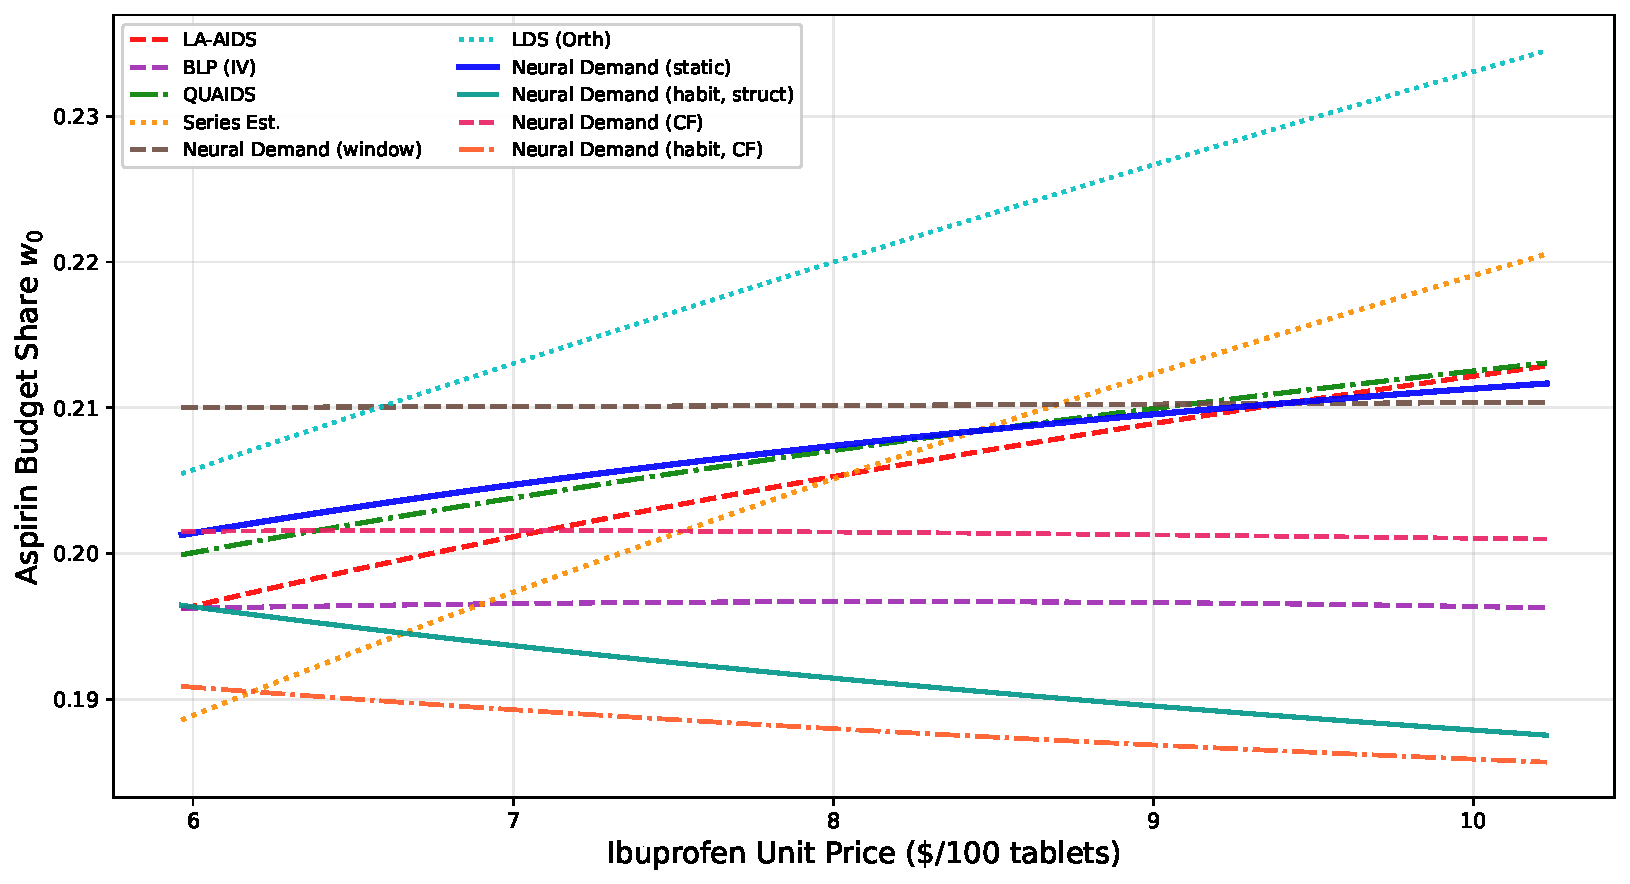
\includegraphics[width=\textwidth]{results/neural_demand/dominicks/figures/fig_demand_curves.pdf}
  \caption{Aspirin Budget Share as a Function of Ibuprofen Unit Price --- Dominick's Analgesics. Shaded bands indicate $\pm 1$ standard deviation across 2 independent re-estimations.}
  \label{fig:dom_demand}
\end{figure}

\begin{figure}[htbp]
  \centering
  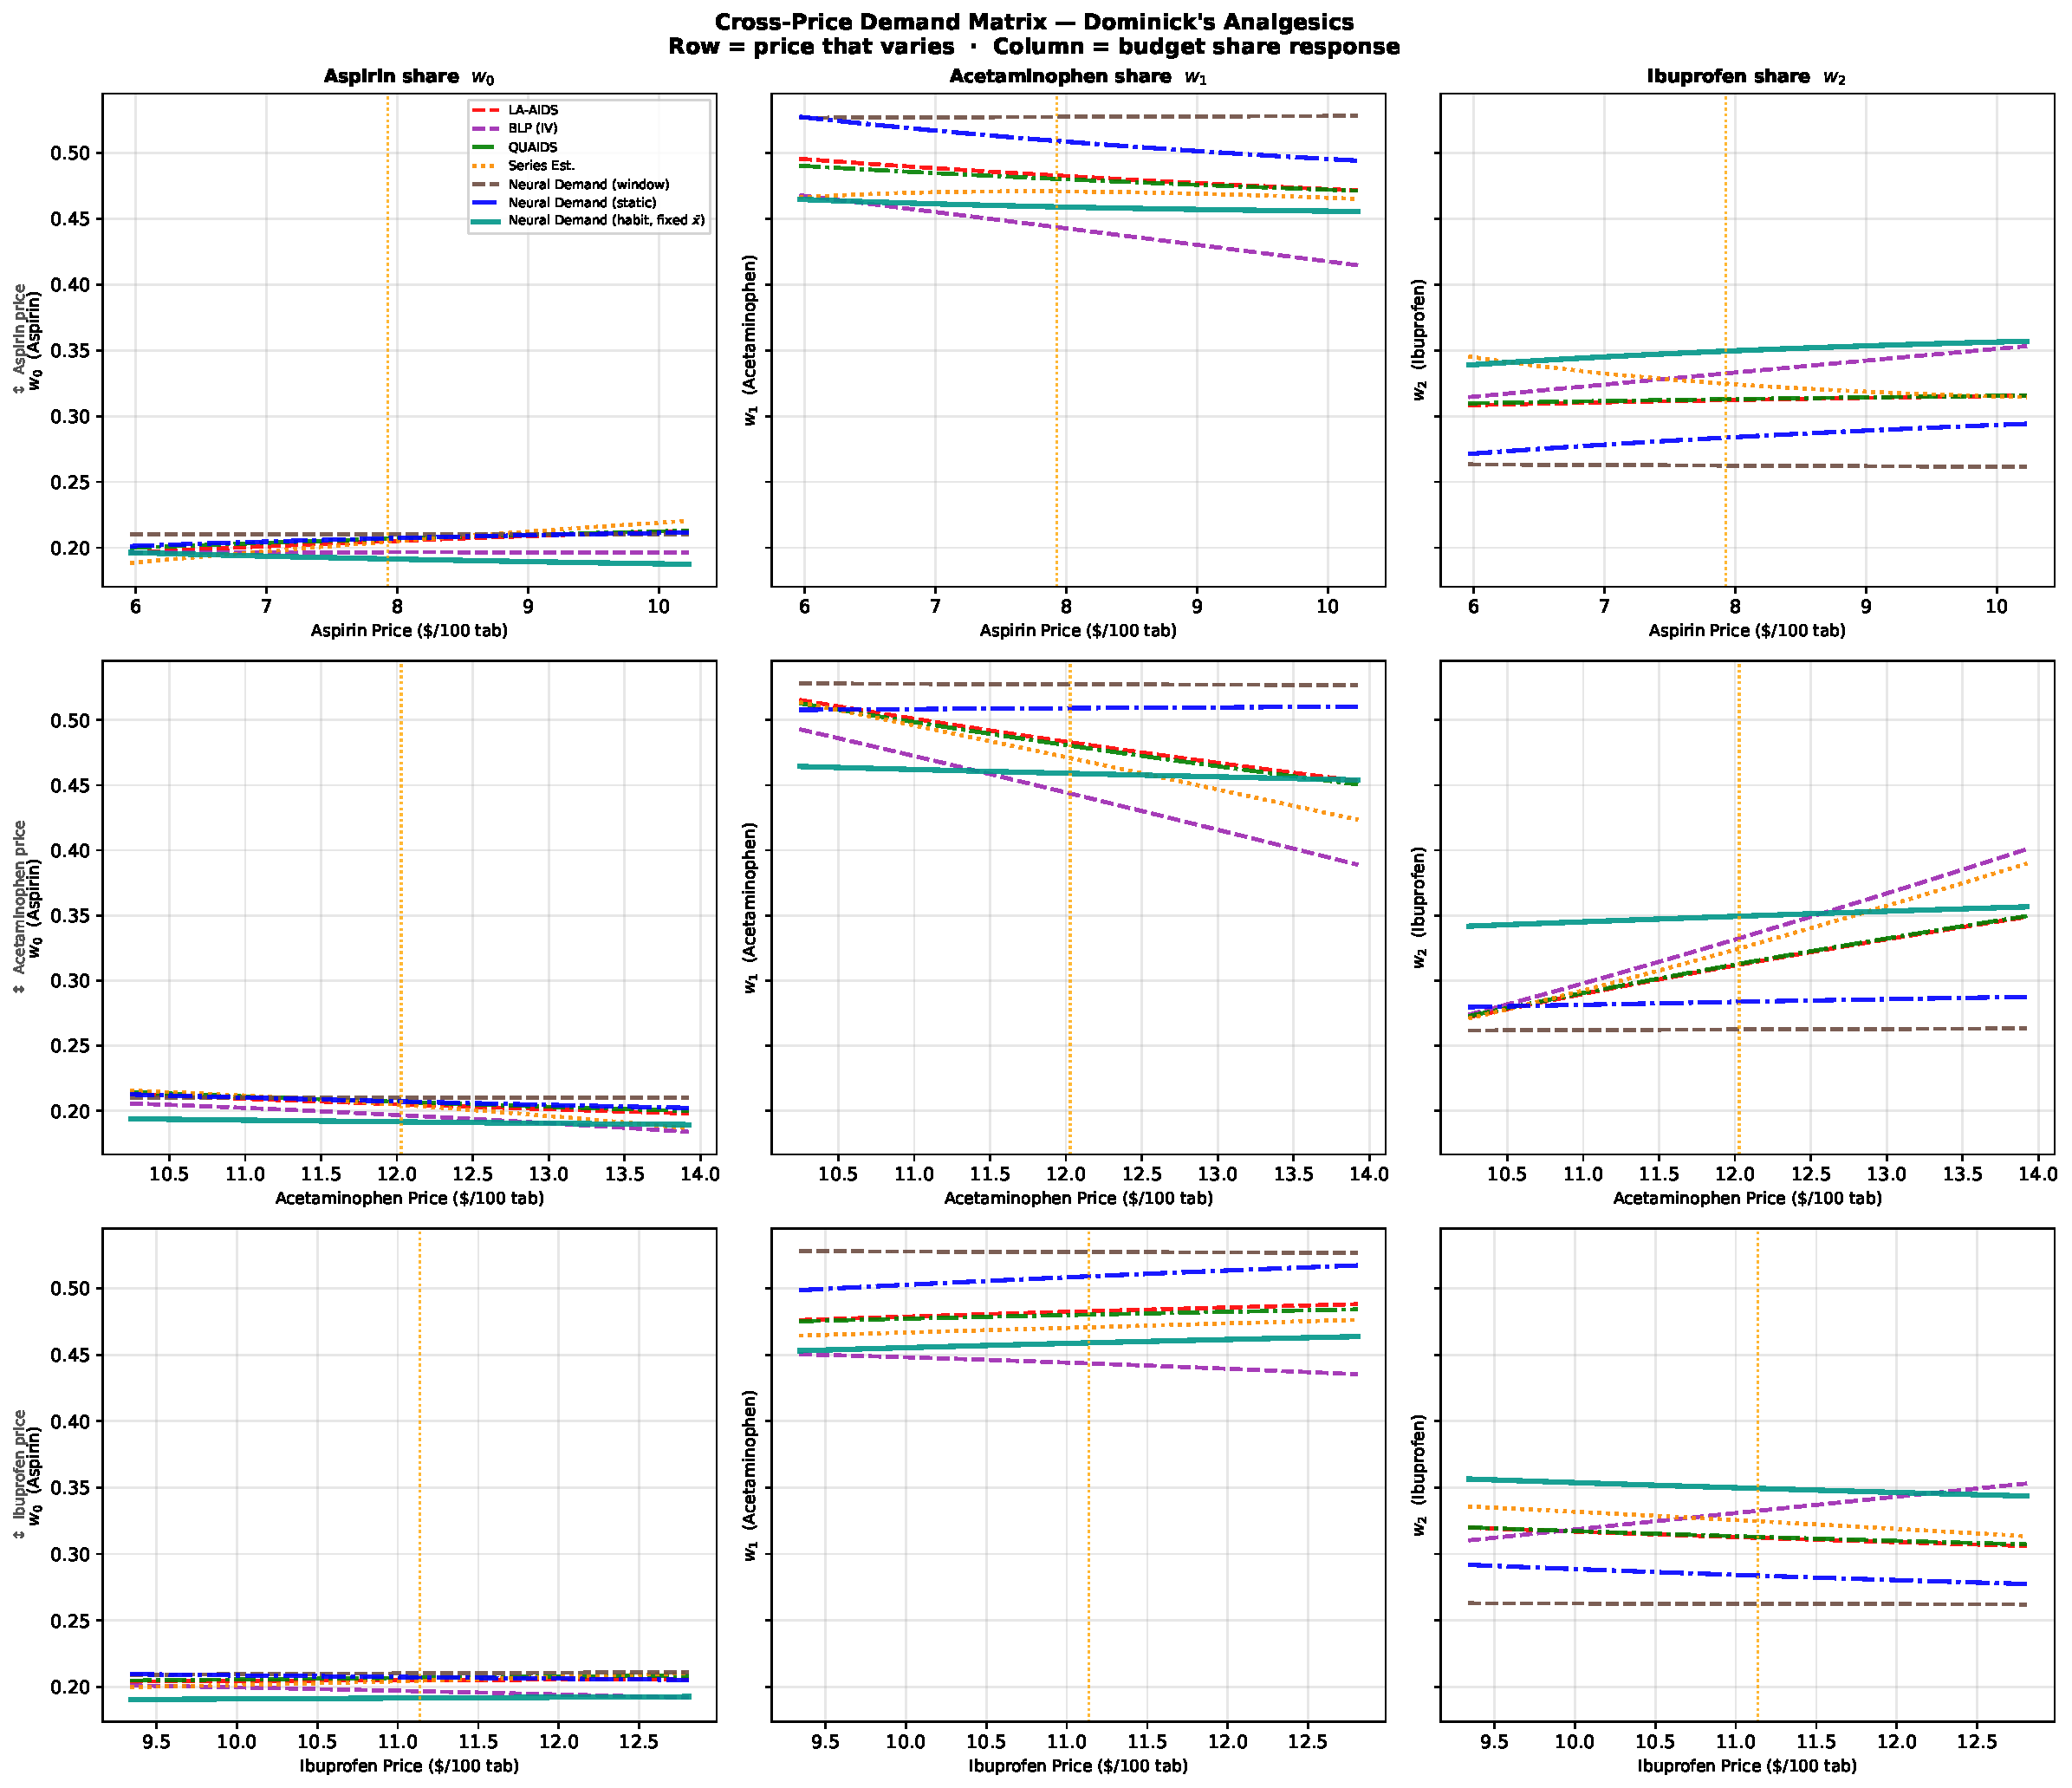
\includegraphics[width=\textwidth]{results/neural_demand/dominicks/figures/fig_mdp_advantage.pdf}
  \caption{Cross-Price Demand Matrix — Dominick's Analgesics. Shaded bands indicate $\pm 1$ standard deviation across 2 independent re-estimations.}
  \label{fig:dom_mdp}
\end{figure}

\begin{figure}[htbp]
  \centering
  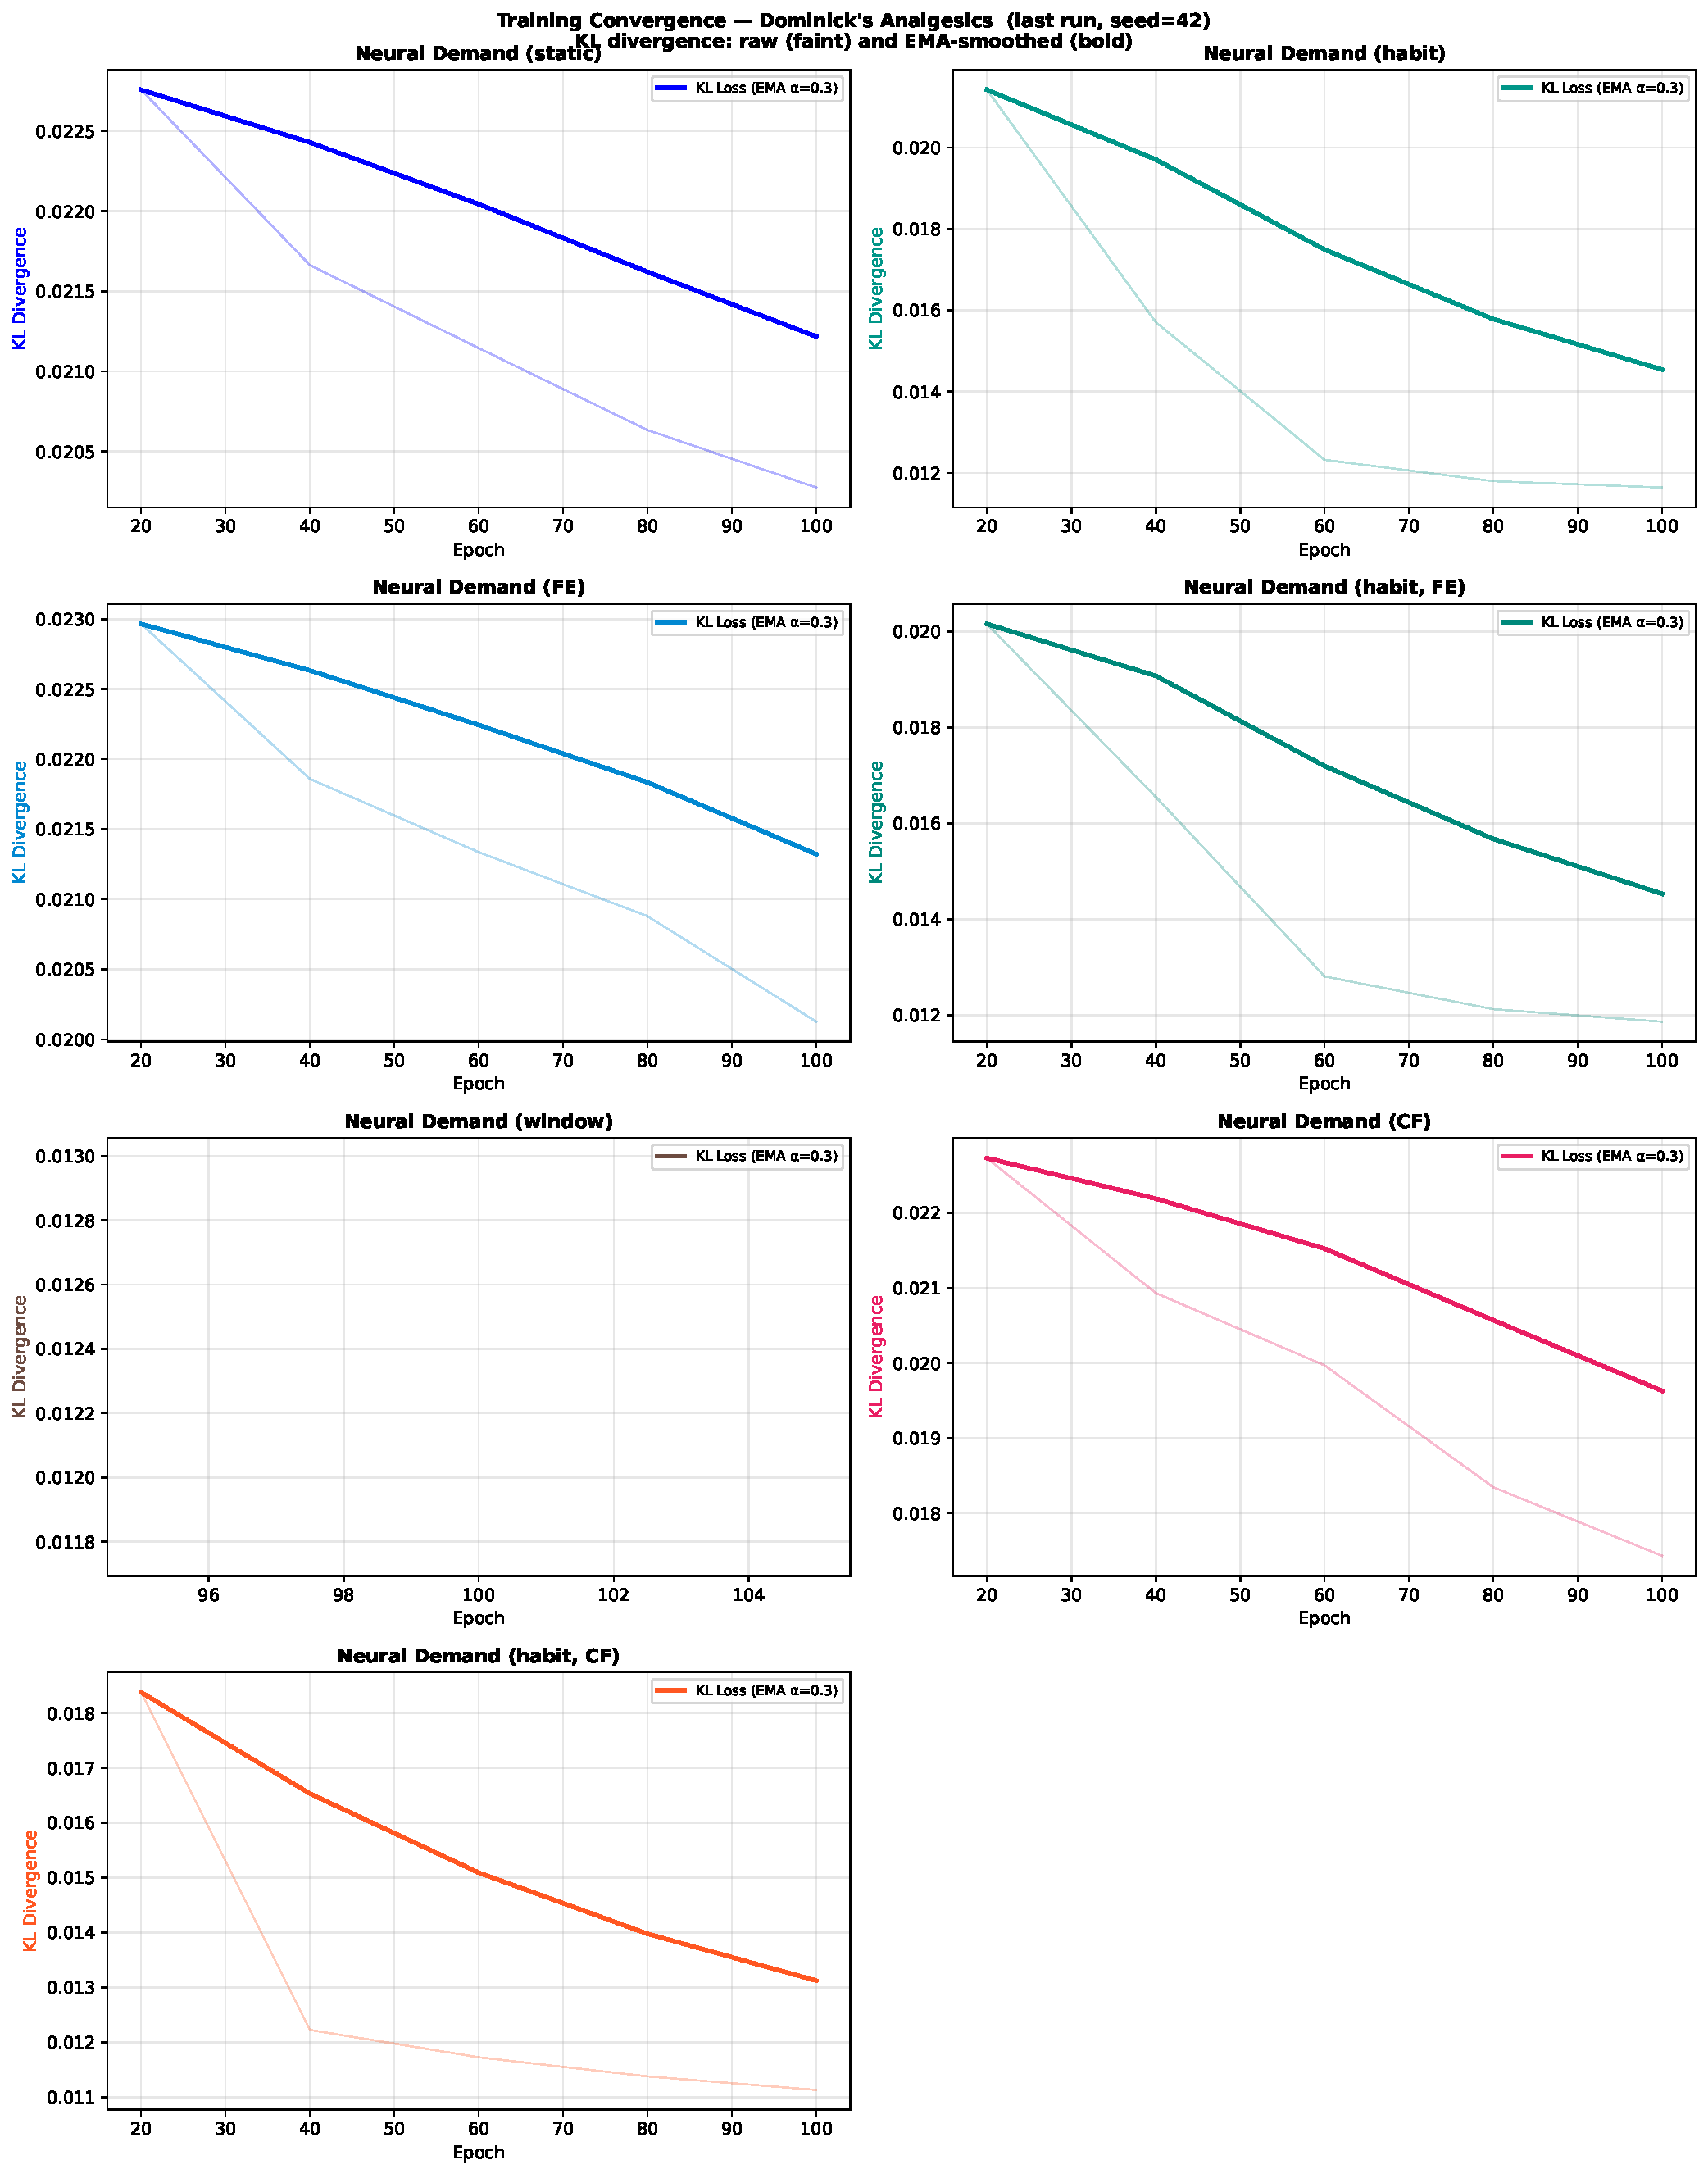
\includegraphics[width=\textwidth]{results/neural_demand/dominicks/figures/fig_convergence.pdf}
  \caption{Training Convergence — Dominick's Analgesics (last run).}
  \label{fig:dom_conv}
\end{figure}

\begin{figure}[htbp]
  \centering
  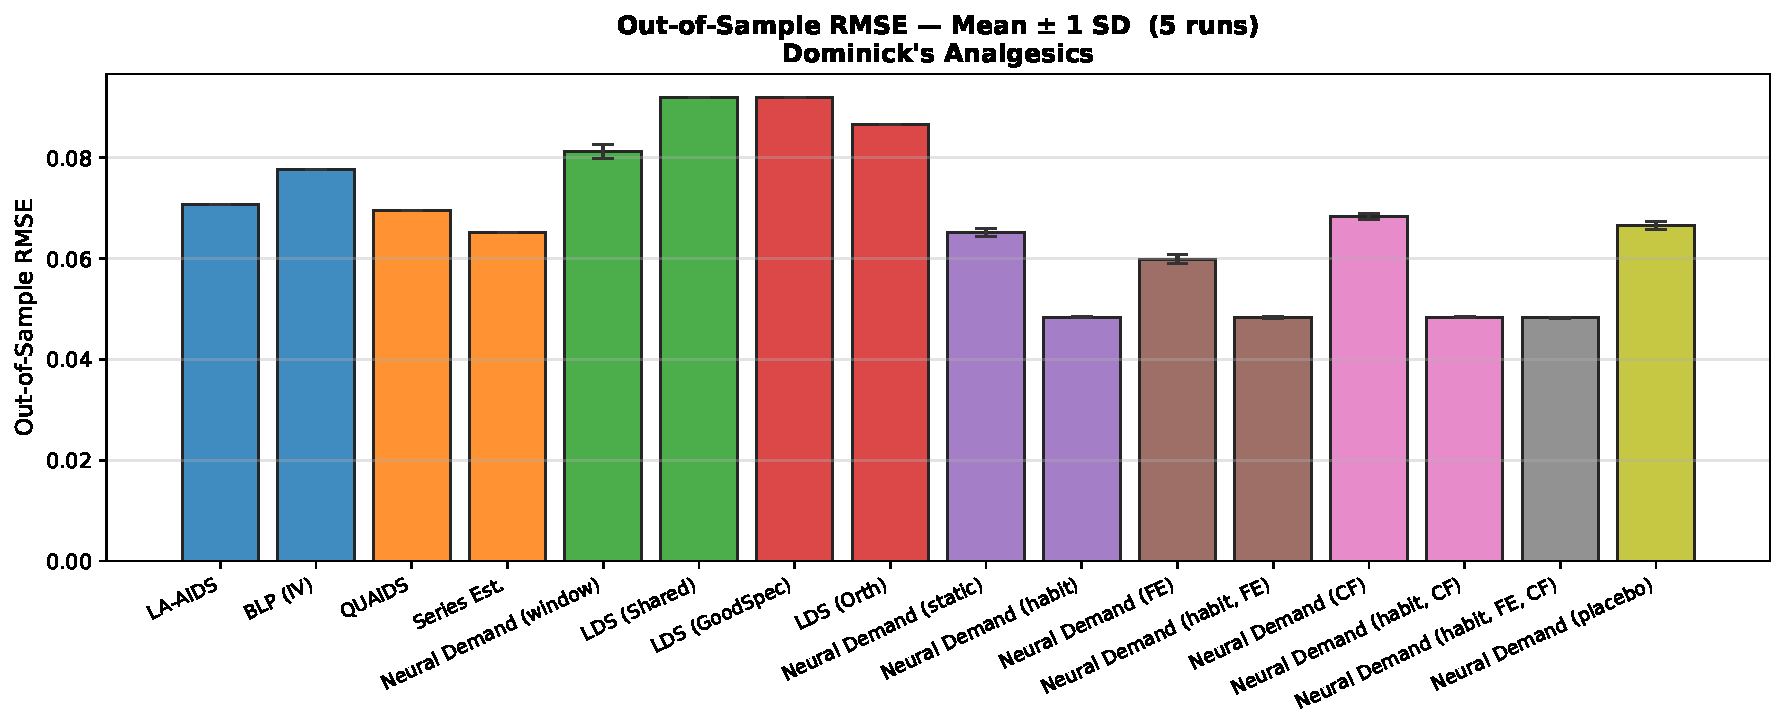
\includegraphics[width=\textwidth]{results/neural_demand/dominicks/figures/fig_rmse_bars.pdf}
  \caption{Out-of-Sample RMSE across all models — mean $\pm 1$ SD over 2 runs.}
  \label{fig:dom_rmse_bars}
\end{figure}

\begin{figure}[htbp]
  \centering
  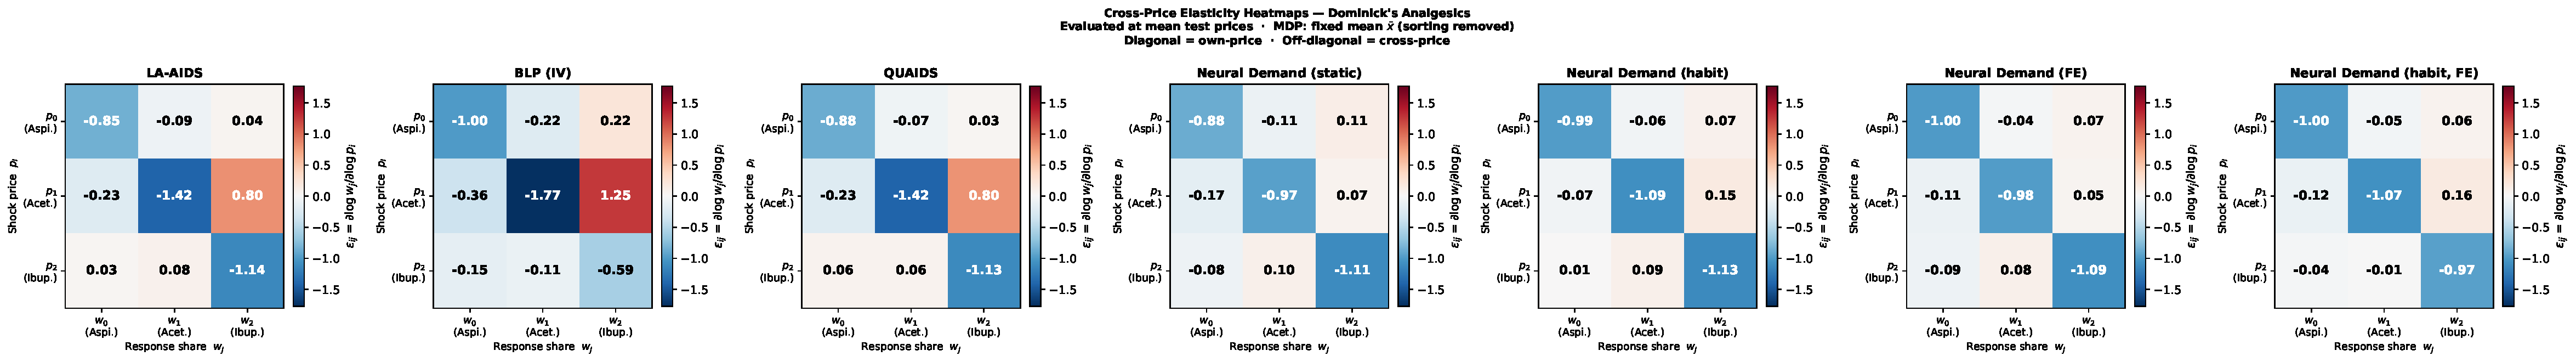
\includegraphics[width=\textwidth]{results/neural_demand/dominicks/figures/fig_cross_elast_heatmap.pdf}
  \caption{Cross-Price Elasticity Heatmaps.}
  \label{fig:dom_cross_elast}
\end{figure}

\begin{figure}[htbp]
  \centering
  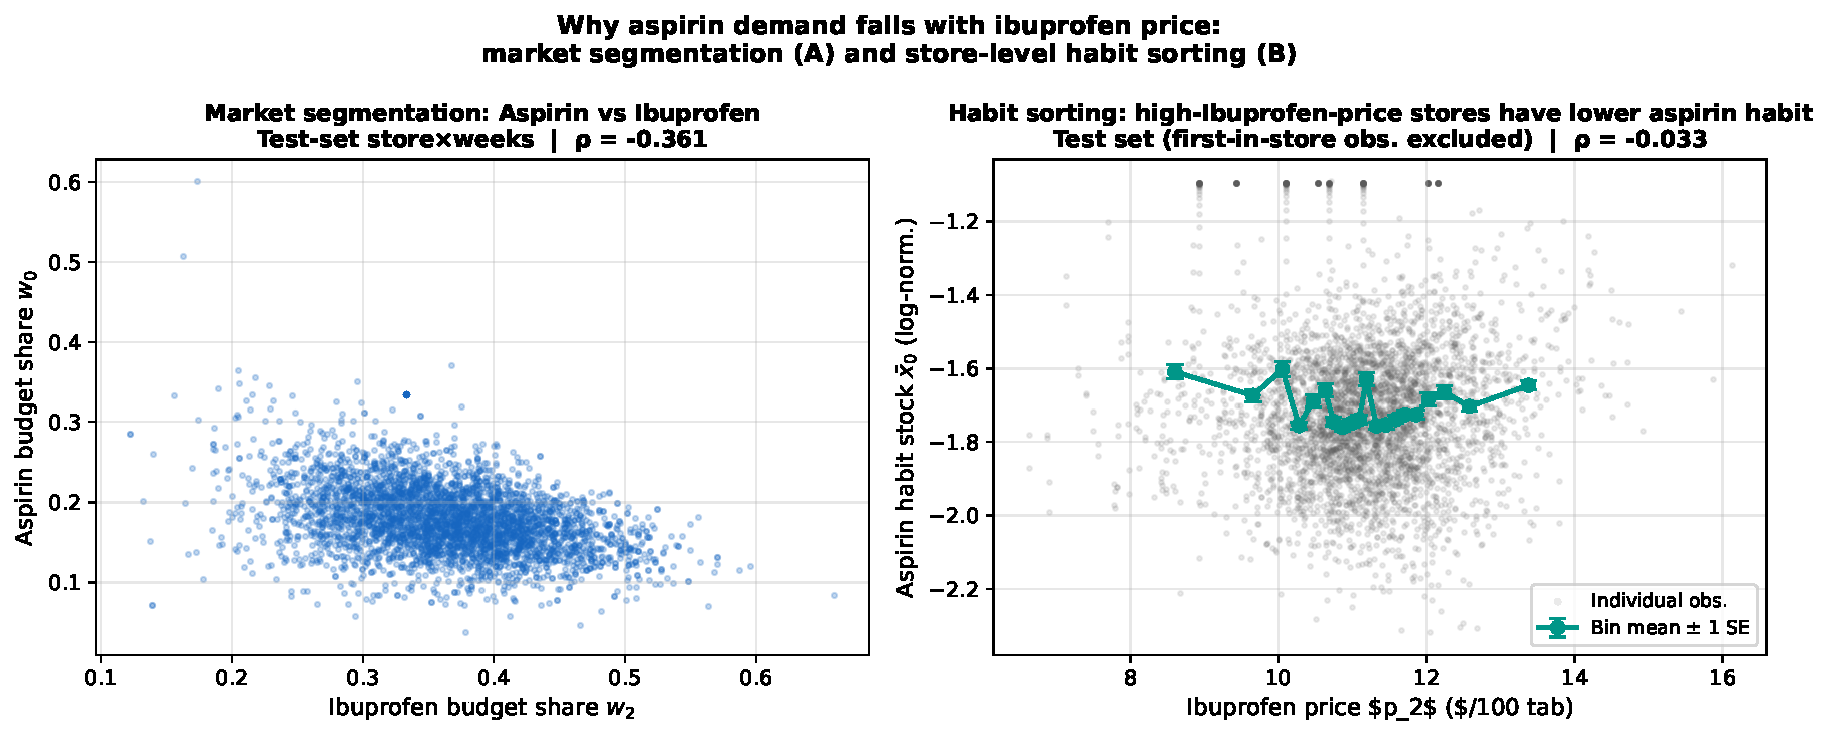
\includegraphics[width=\textwidth]{results/neural_demand/dominicks/figures/fig_segmentation_sorting.pdf}
  \caption{Market segmentation and habit-sorting diagnostics.}
  \label{fig:dom_sorting}
\end{figure}

\begin{figure}[htbp]
  \centering
  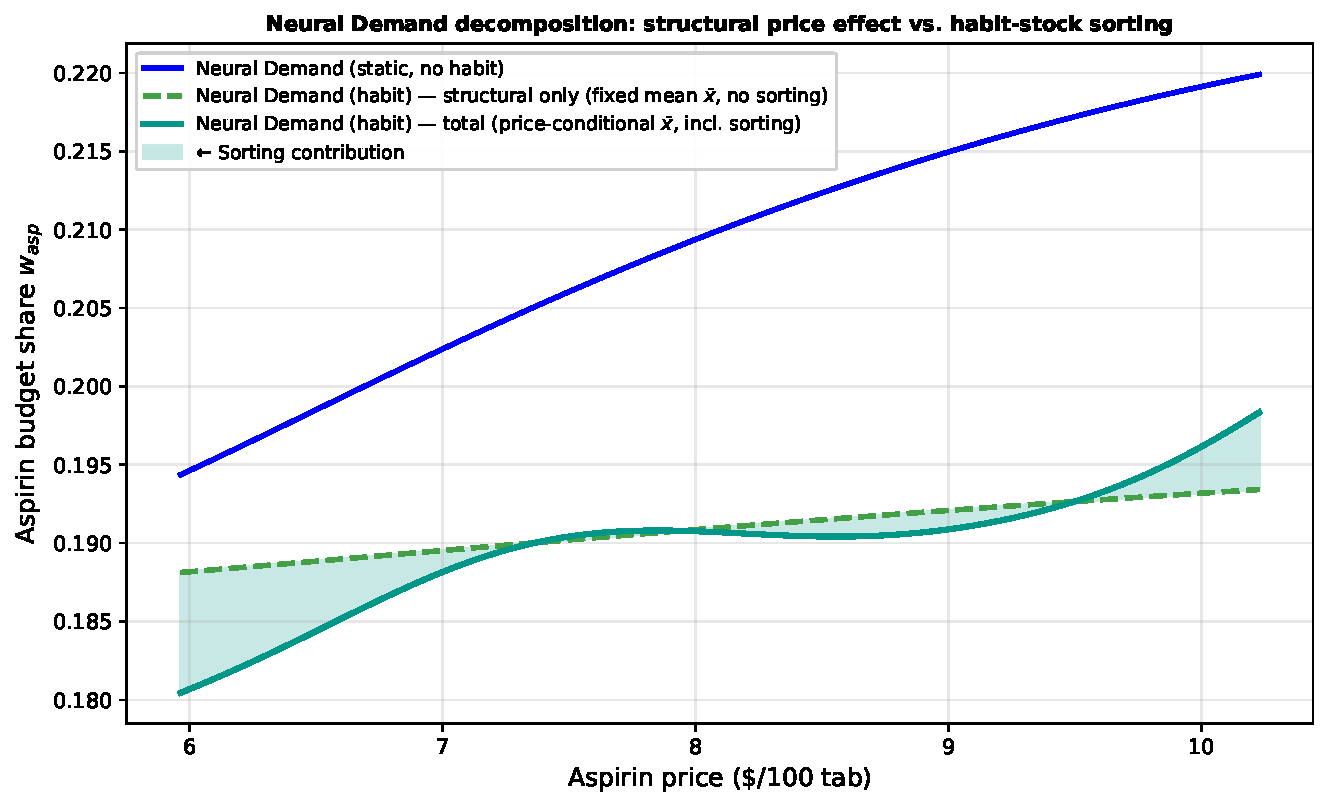
\includegraphics[width=\textwidth]{results/neural_demand/dominicks/figures/fig_mdp_decomposition.pdf}
  \caption{MDP demand decomposition: structural price effect vs. habit-stock sorting.}
  \label{fig:dom_decomp}
\end{figure}
